\chapter{Foundation Models in High-Energy Physics}
\label{ch:foundation_models}

One of the main driving forces behind the successes and widespread adoption of machine learning in natural language processing (NLP) and computer vision (CV) is the utilization of large pre-trained models, often referred to as foundation models (FMs)~\cite{OpportunitiesRisksFoundation}.
Especially for language tasks, most modern applications are built on top of publicly available \textit{pre-trained} FMs, such as BERT~\cite{BERT} or GPT~\cite{GPT, GPT2}, which already possess a basic understanding of language.
FMs are large models typically trained on a large corpus of domain-related data to learn expressive, but generic representations of the subject.
Copies of the FM can then be made and trained once more on a specific task.
The initial training stage is known as pre-training.
The second training stage is known as fine-tuning.

Self-supervised pre-training followed by supervised fine-tuning is the standard approach used by the many successful FMs in NLP~\cite{BERT, GPT, GPT2, BART, LanguageModelsAre} and CV~\cite{DINO, Dalle, Flamingo, MAE, BEIT, IJepa}.
Current research in these fields is focused on developing new self-supervised learning (SSL) strategies and improving pre-training efficiency.
Pre-training tasks in NLP typically involve predicting the next token in a sequence, as with GPT, or randomly masked tokens, as with BERT.
Common \textit{downstream} tasks include sentiment analysis and machine translation. The FM in these tasks is also referred to as the \textit{backbone} as it contains most of the trainable parameters, though additional learnable layers may still be required.

As discussed in this thesis, the field of high-energy physics (HEP) has increasingly integrated machine learning (ML) methods to tackle diverse challenges, including event reconstruction, anomaly detection, and data generation.
These developments have largely mirrored the trends of the wider ML community: model sizes across all fields have grown exponentially, and transformer-based neural networks have become the dominant architecture for many tasks.
However, HEP has yet to fully embrace the FM paradigm, which could provide a powerful tool for the field, though studies are now emerging that explore this potential~\cite{MPM, MPM2, ReSim, JapanPretrain, Omnijet, Omnilearn, LargeScalePretraining, JetCLR}.

This section describes work done on developing SSL strategies for particles physics jets expressed as sets of constituents, as used in \Cref{ch:spice,ch:jet_generation}.
The initial paper on the topic, \textcite{MPM}, introduced the masked particle modelling (MPM) method and demonstrated that it could be a viable pre-training strategy for jet data.
The follow-up study, \textcite{MPM2}, further refined this method into MPMv2, demonstrating its effectiveness in various downstream tasks.
Code for both studies is publicly available~\cite{MPMCode, MPM2Code} and additional results for this section can be found in \Cref{app:foundation_models}.

\section{Masked Particle Modelling}

Developing a good SSL strategy for HEP data would be particularly advantageous as experimental data is unlabelled.
Many ML models are trained in a supervised manner on simulated datasets, in order to have access to truth labels.
However, running high-quality physics simulations is a time-consuming process, and they don't perfectly model real physics.
This causes a domain shift between the synthetic samples the model was trained on and the real data to which it is then applied.
A good SSL strategy would allow training on the billions of real collision events recorded by the LHC experiments over the past few years.

The most popular SSL strategies can be broadly grouped into invariance-based methods and generative methods~\cite{IJepa}.
Invariance-based methods train an encoder to produce similar embeddings given multiple augmented views of the same sample.
These methods typically require hand-crafted and meaningful augmentations that are specific to the data modality.
In image data, these might correspond to random scaling, cropping, masking, or color jittering; augmentations known \textit{a priori} that do not meaningfully change the content of the sample.
For jet data it is unclear what augmentations would be optimal.
JetCLR~\cite{JetCLR} used approximate, but physically inspired augmentations, such as rotations of the constituents about the jet axis and the smearing of soft constituents to estimate soft gluon radiation.
This works well on simplified datasets, where each jet constituent is expressed as a massless kinematic object, but it is unclear how well it would work on sets of reconstructed tracks as used in \Cref{ch:spice}.
R3SL~\cite{ReSim} is a framework where the multiple views are generated by reusing the same synthetic underlying event duplicated at some point in the simulation pipeline.
The simulation is then completed with different seeds or settings.
While this method results in more physically accurate augmentations, it explicitly requires synthetic data.

Current theory on biological systems suggests that representation learning is driven by the need for an internal model that can predict sensory input changes~\cite{cognitivelearning}.
This has led to the development of many models which fall into the second category of SSL, known as generative methods.
These methods involve corrupting or removing parts of the input sample and training the model to predict the missing content.
Such methods can be framed within the context of denoising autoencoders (DAE)~\cite{DAE}.
In a DAE, a lossy augmentation is first applied to the inputs, which are then projected via an encoder into a latent space.
Subsequently, a decoder maps this latent representation to the original, uncorrupted signal.
Only the encoder is retained post-training for further applications, while the decoder is usually discarded.

For a DAE, one hyperparameter is the level and type of corruption applied to the input.
Masking or simply removing a fraction of elements from the input set is a simple, efficient, and effective corruption technique that underpins several notable models in NLP and CV.
Unlike designing specific augmentations, it requires minimal prior knowledge of the domain and applies to many fields.
This is the approach taken by our method, MPM.

\subsection{Overview of Methods}

The objective of the MPM is to develop a model capable of inferring the attributes of the original particles within the masked set, utilizing information from all other particles in the jet.
The representation of a jet as set of particles, each characterized by continuous features, fits well within the masked training paradigm similar to masked language models such as BERT~\cite{BERT}.
However, the MPM scheme is suited for unordered set-based data rather than the sequential data used in NLP.
Another notable challenge arises from the continuous nature of particle features, which contrasts with the discrete dictionaries in language models.
It is similar to the challenges encountered when masking image patches in computer vision.
It is addressed by developing an additional model to discretize or \textit{tokenize} the data using methods similar to those used in BEiT~\cite{BEIT}.

\subsubsection{Masked Particle Modelling}
\label{subsec:mpm}

Jets with $N$ constituent particles are described as a set $\mathcal{X}=\{\x_i\}_{i=1}^N$, where each $\x_i$ represents the attributes of a single particle.
In MPM, $M$ particles out of the $N$ that constitute the jet are selected using some predefined masking strategy.
All selected particles are replaced with a learnable vector called the mask token $\m$.
This new set of surviving particles and mask tokens $\mathcal{S}=\{x_i\}_{i=1}^M~\cup~\{\m\}_{1}^{N-M}$ is fed into a model to recover the original set.
An encoder is used to map the set $\mathcal{S}$ into a latent space, and a prediction head is used to predict the original attributes of the masked particles.
A per-particle loss is used which is only calculated over the masked elements of the set.
A rough outline of the intended pre-training process is shown in \Cref{fig:mpm1}.

Unlike language models, which operate on a finite and discrete vocabulary, many features describing particles are continuous, such as momentum.
This distinction influences two key aspects of the model.
In terms of model input, continuous features can be used directly, as seen in CV, or they can be discretized by binning each feature dimension and using the bin index as an input token, as seen in \textcite{JetGPT}.
In terms of model targets, missing particle features can be used directly, but if discretised, then the model could simply predict the index of the bin containing the missing feature.
This choice of targets also impacts the pre-training loss function.
Predicting continuous features typically involves a regression-type loss, while predicting discrete indices frames this task as a classification problem, enabling the model to learn a categorical posterior distribution over indices.
Modelling the full posterior distribution can prevent the model from focusing on irrelevant details.
Discrete and continuous representations for both input and output is compared.

Particles forming a jet are permutation invariant, making it natural to use a permutation equivariant backbone model.
However, using the same learnable vector $\m$ for all particles in the masked set makes the model's output identical at every masked position, resulting in degeneracy that can only be eliminated by inducing ordering or adding attributed inter-particle connections.
This redundancy prevents zero-error prediction unless all masked particle values are identical.
Despite this, MPM remains valuable because learning the marginal density over the masked set is challenging.

Two strategies address this degeneracy.
One is to define an ordering of the particles and use absolute positional encoding as defined in \Cref{sec:edge_biases_sequences}.
This would compromise the desired permutation invariance of the backbone.
This ordering can be based on any particle attribute; transverse momentum is a reasonable choice.
However, since the task is to recover the particle's dropped features, including the momentum, the model could achieve this by simply examining the particle's location within the sequence.
This is not an issue in images or text, where the sequence position does not directly define a dropped attribute.

Another strategy is to provide this positional encoding only at the input of the masked prediction head.
This breaks the degeneracy in the loss while preserving the backbone's permutation invariance for downstream tasks.
The masked prediction head is a simple MLP with no interactions between elements in the set.
The following approaches are compared: allowing this degeneracy, adding positional encoding to the backbone, and adding positional encoding to the prediction head.

\begin{figure}
    \centering
    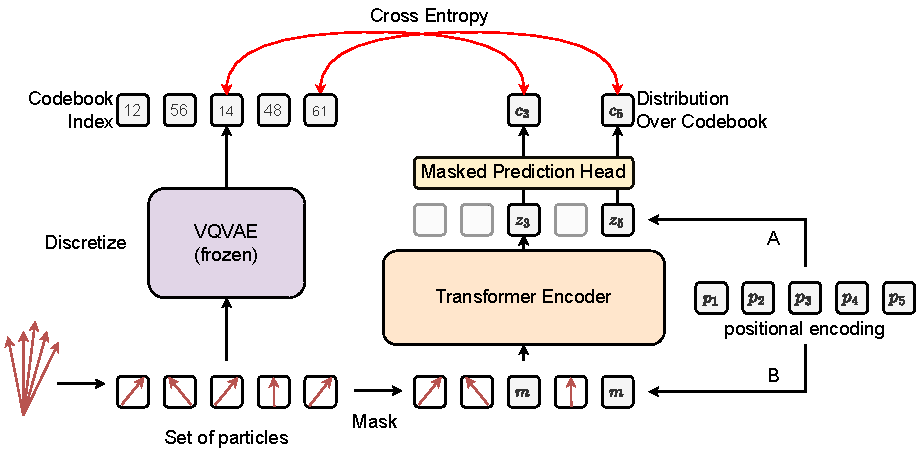
\includegraphics[width=0.99\linewidth]{Figures/foundation_models/mpm1.pdf}
    \caption{
        The proposed model and training scheme for MPM.
        Jets are represented as a set of particles, and some are selected to be replaced by masked tokens and passed through a transformer encoder.
        Training aims to predict the discrete token identity, defined by the output of a pre-trained VQVAE, of the masked particles.
        Positional encoding can be used in the prediction head (A), or in the backbone inputs (B).
    }
    \label{fig:mpm1}
\end{figure}

\subsubsection{Making Tokens From Particles}
\label{subsec:vqvae}

An effective tokenization scheme is essential to evaluating the impact of using discretized representations for either inputs or targets.
The most straightforward approach involves binning each feature using a finite set of ranges~\cite{JetGPT}.
More performant than binning, is discretization via the K-Means algorithm~\cite{KMeans}, whereby each cluster is assigned a unique index.
Both of these methods discretize constituents based on their raw features, but lack contextual information regarding particle features relative to the rest of the jet.

A Vector Quantized Variational Auto-Encoder (VQVAE)~\cite{VQVAE} is used for a context-dependent tokenization scheme.
A VQVAE requires a predefined number of codebook vectors.
An encoder maps inputs to latent vectors, which are individually replaced with the nearest codebook vector, and a decoder reconstructs the original input from these quantized latent vectors.
A transformer is used as both the encoder and decoder.
Even though each embedded particle is quantized independently, the embedding itself, therefore, depends on all particles in the jet.

\subsubsection{Fine-Tuning}
\label{subsec:fine-tune}

Evaluating the utility of a pre-trained backbone requires suitable downstream tasks for benchmarking.
This work focuses on jet classification in various contexts.
This task requires attaching new, randomly initialized, layers to the end of the pre-trained backbone.
As jet classification is a graph-level task, it requires a pooling operation to reduce the set of particles to a single vector.
In the following experiments a learnable weighted pooling operation followed by a linear layer to match the number of jet classes is applied.

Three strategies are examined for training a model for a downstream task:

\begin{itemize}
    \item \textbf{Fixed backbone}: The weights of the pre-trained backbone are frozen during the supervised task and only the linear classification head updated. This tests the linear separability of fixed representations.
    \item \textbf{Fine-tuned}: Both the linear classification head and backbone model are updated. This is the standard fine-tuning procedure and evaluates the utility of pre-training for initializing the model's weights.
    \item \textbf{From scratch}: The backbone model is reinitialized with new, random, weights and fit directly on the downstream task, providing a performance benchmark without pre-training influence.
\end{itemize}

\subsection{Data}
\label{sec:mpm_data}

MPM does not require labels and can be directly applied to experimental data.
However, due to the lack of readily accessible large open datasets of real jets (at the time of writing), MC simulations are used to develop the framework.
All truth labels are ignored during pre-training, but are used to evaluate the model's performance on downstream tasks.

The main dataset in this study is the publicly available JetClass dataset~\cite{JetClass}; with 125 million jets across 10 classes (100M for training, 5M for validation, 20M for testing).
Jets in this dataset are fat jets, \Cref{sec:fat_jets}, comprising multiple quark or gluon jets overlapping due to highly boosted decays.
Each class represents jets captured when simulating specific decay chains, such as $H \rightarrow b\overline{b}$, and $t \rightarrow b \ell \nu$.
Events are generated using \pythia~\cite{Pythia8}, with top, $W$, $Z$, and Higgs decays modelled with \madgraph~\cite{MadGraph}.
Detector simulation is performed using \delphes~\cite{Delphes} and is configured to match the CMS experiment.
Jets are reconstructed using calorimeter energy deposits with the anti-$k_T$ algorithm~\cite{AntiKt} with the radius parameter set to $R=0.8$.
Jets are selected to have roughly the same transverse momentum $\pt$ distribution across all classes, ranging from $500$ to $1000~\GeV$.
On average, each jet contains 50 particles, with a maximum of 120.

Each particle is virtually massless and described by its transverse momentum $\pt$, pseudo-rapidity to jet axis $\Delta\eta$, and azimuthal angle to jet axis $\Delta\phi$.

\subsection{Model Architecture}

The same transformer encoder architecture is used as the backbone in all experiments.
Eight TE Blocks based on the Normformer architecture~\cite{Normformer} are used with a model dimension 1024, comprising a total of 40 million parameters.
Input particles are linearly embedded into the model dimension.

After passing through the backbone, the output nodes are used in dedicated layers called \textit{heads}.
The pre-training head consists of a single MLP applied per node, followed by a softmax for classification or a linear layer for regression.
The fine-tuning classification head is a weighted average over all output dimensions, followed by another linear layer and softmax.

All models are trained with the AdamW~\cite{AdamW} optimizer with a weight decay of $0.01$.
Pre-training is performed over five epochs on the full JetClass dataset.
For supervised fine-tuning, all models are trained for up to 50 epochs with early-stopping enabled.
In both settings the learning rate is ramped up linearly from zero to $10^{-4}$ over 1k steps and the norm of the gradients is clipped to 1.0.

A codebook of size 512 is used for the VQVAE and 512 centroids are used for the K-Means.
For the masking strategy, the mask rate $D_f=\sfrac{M}{N}$ is fixed to 0.3, meaning 30\% randomly selected particles in the jet were masked.
Each particle has equal probability of being masked.

\subsubsection{VQVAE Training}

A VQVAE consists of an encoder $F$ and decoder $G$, a quantization layer $h$, and a codebook ${C}=\{c_i\}_{i=1}^m$ for vectors $c_i \in \mathbb{R}^n$ where $n$ is the latent space dimension.

The quantization layer $h: \mathbb{R}^n \times {C} \rightarrow c \in {C}$ acts on a latent vector by assigning it to the closest codebook element based on the Euclidean norm as the distance measure.
The codebook $C$ will always be omitted from the arguments of the function $h$ in the following.
The output of a VQVAE is defined as,
\begin{align}
    \hat{x} & = G(h(F(\x))) \\
            & = G(h(\z_e))  \\
            & = G(\z_q),
\end{align}
for a given input $\x$.
The objective of a VQVAE is typically to minimize the reconstruction measure in the input space.
Gradients for this loss can not be backpropagated to the encoder, as the operation $h$ is not differentiable, and have to be estimated using the straight-through estimator~\cite{StraightThrough}.
An extra commitment loss term is included to create an attractive force between the encodings $(z_e=F(x))$ and their corresponding codebook vectors $(z_q = h(z_e))$,
\begin{equation}
    \mathcal{L}_{cmt} = (1-\beta)d(z_e,\mathrm{sg}(z_q)) + \beta d(\mathrm{sg}(z_e),z_q),
\end{equation}
where $\mathrm{sg}$ is the stop gradient operator and $d$ is the Euclidean distance.
The commitment loss is weighted by added to the reconstruction loss with a relative weight of 10 and $\beta=0.9$.

Training a VQVAE~\cite{VQVAE} can be challenging.
One of the main issues is the collapse of the codebook, where all latent vectors are assigned to a single codebook element.
Several best practices are employed to mitigate this issue~\cite{bettervqvae} via the library \texttt{vqtorch}~\cite{VQTorch}.
A shared parameterization is used for all codebook elements with a latent dimension of $n=16$ and the commitment loss only applied every four steps.
The codebook elements are initialized using the K-Means clustering algorithm on the latent space at the start of training.
Specific codebook elements which have not been used for 100 consecutive steps are reinitialised.
Post-training, the codebook achieves approximately 80\% utilization.

The input nodes are each quantized and decoded separately.
A jet with $N$ constituent particles is assigned to $N$ codebook elements which are then decoded to $N$ vectors.
The encoder and decoder follow a similar structure to the backbone with the following modifications.
Only four layers are used in each, and the model dimension is reduced to 256.

\subsection{Experiments}

The first set of experiments are conducted to test the model design.
These experiments aim to understand the impact of tokenization on the input and target features, examine the quality of tokens learned by the VQVAE, and test the effect of the positional encoding.
These are followed by experiments to evaluate the performance of the models on downstream classification tasks.
The tasks include:
\begin{itemize}
    \item In-distribution prediction, where predictions are made using the same classes seen in pre-training
    \item Out-of-distribution (OOD) prediction, where predictions are made using the classes not seen in pre-training
    \item Weakly supervised prediction, where a CWoLa style classifier is trained using noisy labels as described in \Cref{sec:drapes}
\end{itemize}
All experiments are repeated five times with different seeds, and the mean and standard deviation of the results are reported.

\subsubsection{Token Creation with a VQVAE}

To ensure that latent space codes sufficiently capture essential information about particles in a jet, the quality of decoded jet properties after encoding and quantization in the VQVAE is examined.
\Cref{fig:vq_vae} shows that the distributions of decoded jet transverse momentum and mass align well with the input distributions.

\begin{figure}[htp!]
    \centering
    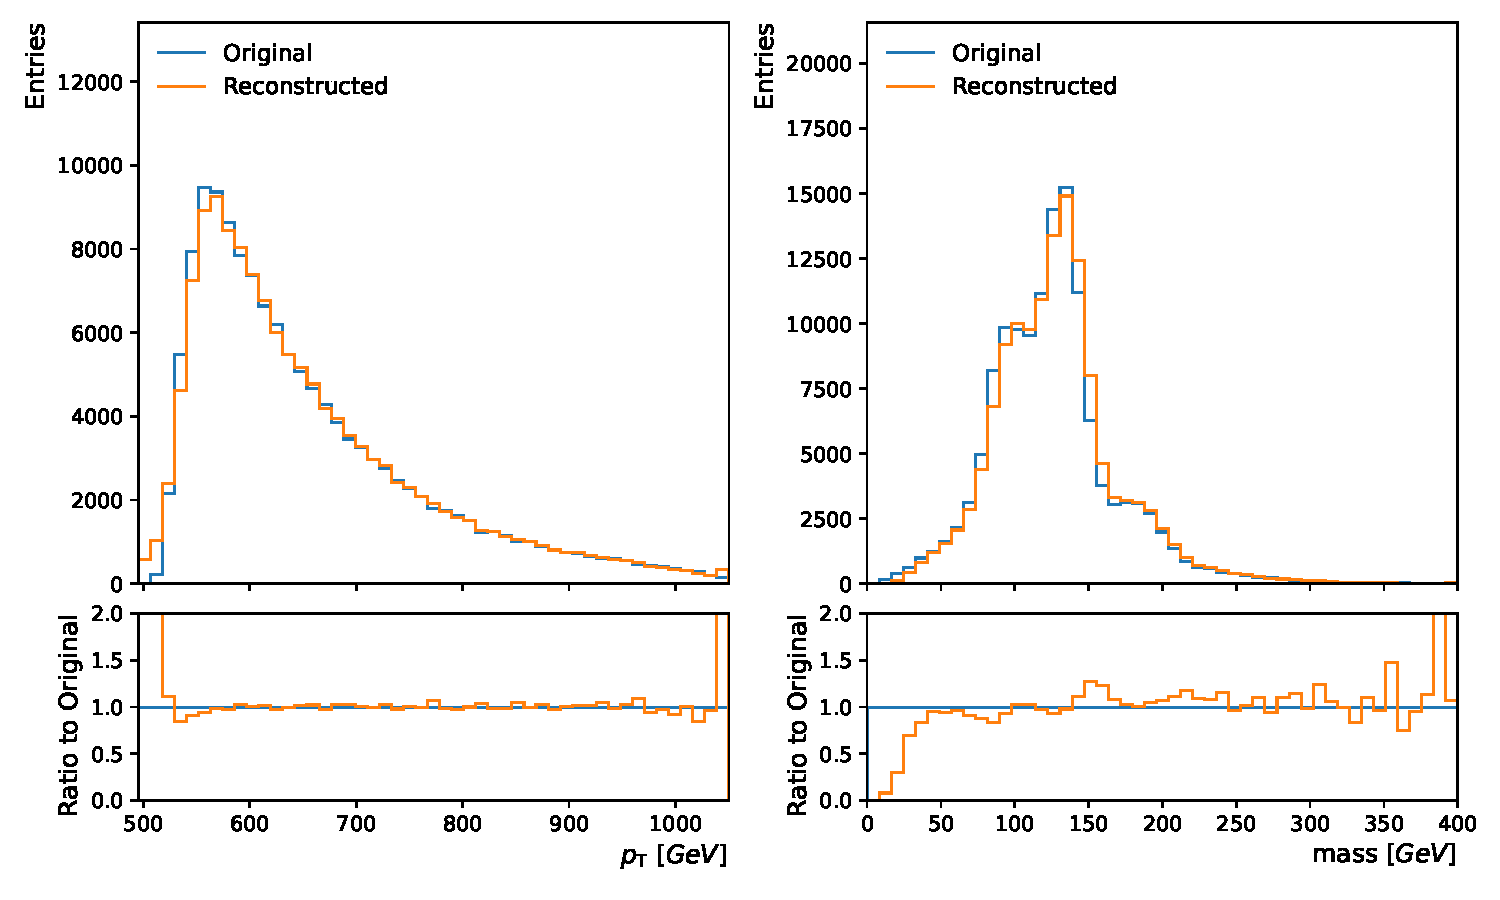
\includegraphics[width=0.8\textwidth]{Figures/foundation_models/mpm1/jet_high_img.pdf}
    \caption{
        \label{fig:vq_vae}
        The reconstruction of the jet mass and transverse momentum using the VQVAE.
    }
\end{figure}

\subsubsection{Discretization and Positional Encoding}

This section examines the pre-training configuration, focusing on the impact of positional encoding, input tokenization, and target tokenization.

Sequence order is defined by decreasing particle transverse momentum, and is expressed using absolute positional encoding (APE).
When a tokenized representation is used for the target, the model is trained using cross-entropy over the codebook indices.
Otherwise, the mean squared error is used as a regression loss.

After pre-training, the backbone is fixed and a linear classifier is trained using the same dataset.
The accuracies are quoted in \Cref{tab:pretraining_compare}.
Applying APE in the model head demonstrates a clear advantage over providing it to the backbone inputs or not ordering at all.
Input quantization negatively impacts model performance due to the information loss.
Using tokens from either the VQVAE or K-Means as classification targets is substantially better than regressing particle features as a prediction task.
Regression offers only a point prediction of average particle properties under the posterior, which has limited predictive power for multi-modal posteriors.
Classification loss is more flexible, allowing for the prediction of the full distribution over tokens.
VQVAE tokens outperform K-Means tokens for classification, likely due to the VQVAE's richer latent space.
However, K-Means tokens perform reasonably well and may be a useful avenue for additional tests, especially due to the ease of implementation compared to the VQVAE.

Following these results, all subsequent tests use a backbone with original continuous inputs, and perform pre-training with APE in the prediction head and use VQVAE tokens as targets.

\begin{table}[htp!]
    \centering
    \caption{Linear probe accuracy on the ten classes of JetClass using backbones with different pre-training strategies. The accuracy is averaged over five different runs with errors on the order of $0.01\%$.
    }
    \label{tab:pretraining_compare}
    \begin{tabular}{lllc}
        \toprule
        Inputs            & Targets        & APE           & Accuracy          \\
        \midrule
        \textbf{original} & \textbf{VQVAE} & \textbf{head} & $\mathbf{56.8\%}$ \\
        original          & K-Means        & head          & $56.2\%$          \\
        original          & VQVAE          & none          & $54.1\%$          \\
        original          & VQVAE          & backbone      & $53.4\%$          \\
        VQVAE             & VQVAE          & head          & $51.1\%$          \\
        VQVAE             & K-Means        & head          & $49.3\%$          \\
        original          & original       & head          & $48.9\%$          \\
        original          & original       & backbone      & $46.3\%$          \\
        \bottomrule
    \end{tabular}
\end{table}

\subsubsection{In-Distribution Classification}

The utility of the backbone model for downstream tasks is first tested on in-distribution data, where fine-tuning is performed on the same dataset as pre-training
The accuracy of the linear classifier is measured on a holdout test set.
Given enough labelled data and sufficient training time, it is expected that any supervised model will converge to a similar as one that is pre-trained.
Therefore, to assess how pre-training makes the model more data-efficient, the number of labelled samples used for fine-tuning is varied.

\Cref{fig:fine_tune_jetclass} shows that with labelled dataset sizes under 10k jets, pre-training offers a significant performance advantage.
This demonstrates the utility of the representation learned during pre-training for downstream tasks.
With a sufficiently large labelled dataset, the supervised model surpasses the fixed backbone model and matches the performance of the fine-tuned backbone model as expected.
Overall, pre-training provides a strong set of initial weights for fine-tuning on downstream tasks.

\begin{figure}[tp!]
    \centering
    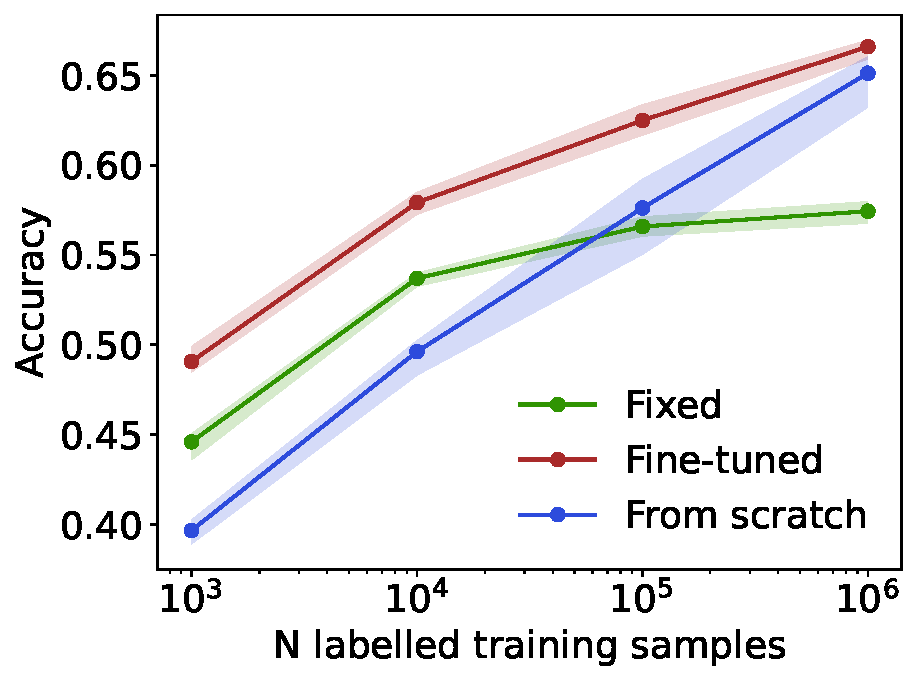
\includegraphics[width=0.5\textwidth]{Figures/foundation_models/mpm1/jc_corrected_pt_40_accuracy.pdf}
    \caption{
        Accuracy of training strategies as a function of the number of labelled samples. Uncertainty bands depict variability in five runs with different seeds.
        ``Fixed'' denotes models with frozen pre-trained weights; ``Fine-tuned'' denotes models with updated weights; ``From scratch'' denotes models with randomly initialized weights.
    }
    \label{fig:fine_tune_jetclass}
\end{figure}

\subsubsection{Out-of-Distribution Classification}

To test whether the pre-trained model learns features useful for tasks on data beyond those seen during pre-training a test on OOD data is performed.
Pre-training is performed on six of the ten classes in the dataset, those pertaining to Higgs, light quarks, and gluons.
Fine-tuning is then performed on the four remaining classes, containing top, $W$, and $Z$ decays.

The results in \Cref{fig:fine_tune_jetclass_ood} show that both pre-trained models, fixed and fine-tuned, outperform training from scratch.
With sufficient labelled data, the fully supervised model surpasses both pre-trained models.

\begin{figure}[tp!]
    \centering
    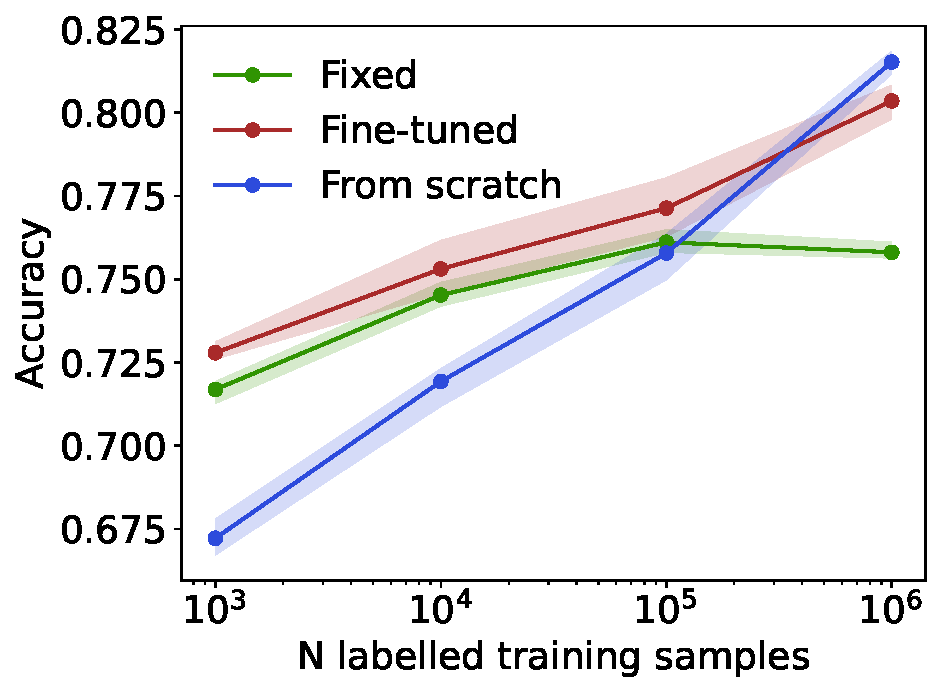
\includegraphics[width=0.5\columnwidth]{Figures/foundation_models/mpm1/jetclass_nc_two_40_accuracy.pdf}
    \caption{Accuracy of training strategies as a function of the number of labelled samples as measured on classes not seen during pre-training.
        Uncertainty bands depict variability in five runs with different seeds.
        ``Fixed'' denotes models with frozen pre-trained weights; ``Fine-tuned'' denotes models with updated weights; ``From scratch'' denotes models with randomly initialized weights.}
    \label{fig:fine_tune_jetclass_ood}
\end{figure}

\subsubsection{Weakly supervised classification}

Fine-tuning tasks are typically supervised and require labels.
Real collider data offers no ground truth labels, but physics knowledge can enrich data from certain decays and final states, providing training data with noisy labels.
These noisy labels can replace or complement fine-tuning with simulated data, leveraging pure labels in simulation and noisy labels in data.
This approach is useful for data-driven weakly supervised search strategies which use these noisy labels to construct a CWoLa classifier as described in \Cref{sec:drapes}.
However, as detailed in that section, the CWoLa classifier struggles with high-dimensional data when using large models like transformers.
Being able to improve their sensitivity via pre-training will make these methods viable for new physics searches.

To emulate the CWoLa setting two datasets are created each containing one million QCD jets.
Next, $N$ samples of another class, top-quark initiated jets, are added to one dataset.
A supervised classifier is trained to discriminate between these datasets and then evaluated on separating QCD jets from top jets.
In \Cref{fig:lp_ws}, significance improvement (SIC) is shown as the ratio of significance before and after applying a 0.5 threshold on the classifier output.
Significance is defined as the number of top jets divided by the square root of the number of QCD jets.
The pre-trained backbone significantly improves the model's performance, even when only the linear head is fine-tuned.

\begin{figure}[htp!]
    \centering
    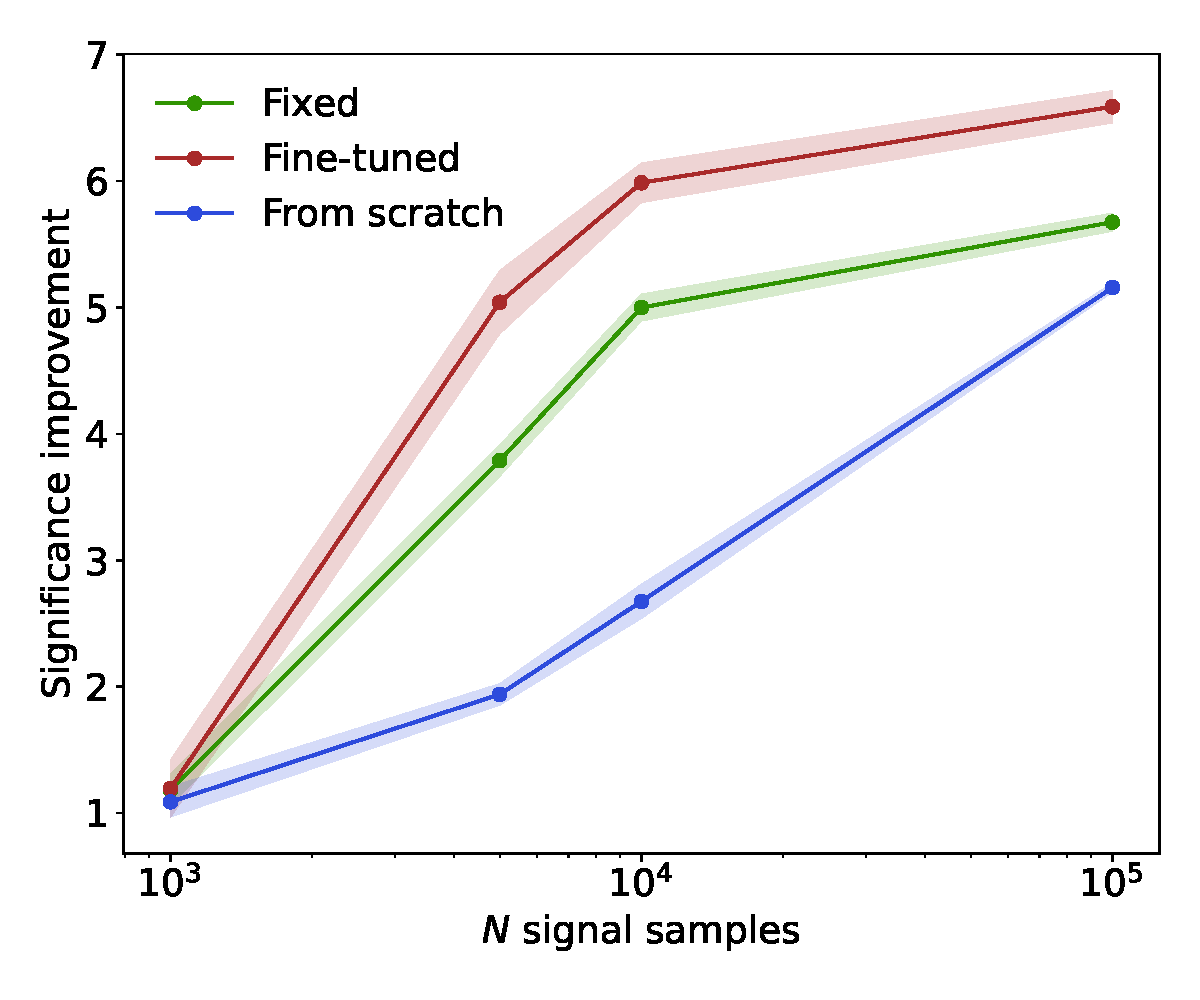
\includegraphics[width=0.5\columnwidth]{Figures/foundation_models/mpm1/cwola_40M_0.pdf}
    \caption{
        Models trained with weak supervision to classify datasets of different label proportions.
        A dataset of one million QCD jets is compared to a dataset with one million QCD jets plus $N$ top jets. Uncertainty bands depict variability in five runs with different seeds.
        ``Fixed'' denotes models with frozen pre-trained weights; ``Fine-tuned'' denotes models with updated weights; ``From scratch'' denotes models with randomly initialized weights.}
    \label{fig:lp_ws}
\end{figure}

\subsection{Conclusion}

The masked particle modelling strategy is proposed for pre-training on unordered sets of inputs and its utility for constructing jet classifiers is demonstrated.
This approach adapts masking strategies from NLP and CV to continuous, unordered particle features.
Pre-training with MPM allows fine-tuned models to perform well on downstream tasks, even with small datasets.
Initial results are promising, indicating that larger pre-training datasets and models could address domain adaptation challenges.
However, models trained from scratch can surpass pre-trained models with sufficient labelled data, highlighting an inefficiency in the fine-tuning process.

\section{Improved Masked Particle Modelling}

In the previous section it was found that a VQVAE leads to a more performant FM than direct regression.
This is argued to be primarily due to two reasons:
\begin{itemize}
    \item The VQVAE latent space is semantically rich, containing high-level abstractions; giving the MPM encoder a more informative target to learn from.
          This is also the justification for using the VQVAE in BEiT~\cite{BEIT}.
    \item By changing from a regression to a classification task, the backbone is taught the full conditional posterior distribution rather than just seeking the mean.
\end{itemize}

However, producing the VQVAE requires an additional training step in the pipeline.
VQVAEs are also notoriously unstable and hard to train.
Furthermore, the quantization leads to a loss of information.

In this follow-up study the following advancements are made:
\begin{itemize}
    \item An improved MPM training paradigm, named MPMv2, is introduced by enhancing model architecture and addressing existing inefficiencies.
    \item The particle attributes are expanded to provide a more detailed representation.
    \item A detailed study of additional reconstruction tasks for MPMv2 pre-training is performed beyond the regression, K-Means, and VQVAE derived tasks from the previous study.
    \item A new test bed is provided that includes a wider set of downstream tasks commonly encountered in jet physics.
\end{itemize}
From henceforth, the original MPM method is referred to as MPMv1.

\subsection{Data}

In addition to JetClass~\cite{JetClass}, a new dataset is introduced, which is labelled as BTag~\cite{btag}.
The BTag~\cite{btag} dataset contains 3 million jets differentiated by their flavour: light, charm, or bottom.

Events are generated using \pythia~\cite{Pythia8}, which also models parton showering and hadronization, and detector response is simulated using \delphes~\cite{Delphes}.
The BTag dataset is different from JetClass in several ways.
They are not large-radius jets, but are reconstructed using the anti-$k_T$ algorithm with a radius parameter of $R=0.4$.
The jets are only required to have $\pt \geq 20~\GeV$, and detector simulation is configured to match the ATLAS experiment instead of CMS.
The final significant difference is that BTag only stores charged particles; thus, they have a much lower cardinality, with a maximum of 15 constituents per jet.

JetClass is utilized exclusively for model pre-training, but both datasets are used for fine-tuning and evaluation.
The discrepancies between these datasets reflect the realistic variations in particle physics jet definitions across different experimental settings.
Targeted kinematic ranges, reconstruction parameters (e.g., anti-$k_T$ radius), and object selection vary significantly based on specific physics analyses and are meticulously tuned by experts.
These differences provide an opportunity to assess the backbone's generalizability to new downstream tasks and an OOD dataset that is further removed than the class separation seen in MPMv1.

The input feature list is expanded to encapsulate all reconstructed attributes that can be found in both datasets.
Charged constituents leave tracks in the detector, so the lifetime signed longitudinal and transverse impact parameters ($d_0$, $z_0$) as well as their reconstruction uncertainties ($\sigma(d_0)$, $\sigma(z_0)$), are included.
Neutral particles do not leave tracks, so these features are zero-padded.
The impact parameters and the three-momentum combine to form the continuous features of the particle, \xc.
Also included is the particle identity (ID) \xid, a one-hot encoded vector that categorizes both the particle type and charge into 8 independent classes.
Each particle is therefore represented by a vector of 8 features, 7 continuous and one categorical, $\mathcal{X} = \{\x_i=(\xc_i, \xid_i)\}_{i=1}^N$, as shown in \Cref{tab:mpm2_inputs}.
The distributions for these features in the two datasets are shown in \Cref{fig:mpm2_features}.

\begin{table}[ht]
    \centering
    \caption{The features used to describe each jet constituent.}
    \label{tab:mpm2_inputs}
    \begin{tabular}[t]{lr}
        \toprule
        \multicolumn{2}{c}{Continuous features \xc}   \\
        transverse momentum           & $\pt$         \\
        pseudorapidity to jet axis    & $\Delta \eta$ \\
        azimuthal angle to jet axis   & $\Delta \phi$ \\
        transverse impact parameter   & $d_0$         \\
        longitudinal impact parameter & $z_0$         \\
        uncertainty on $d_0$          & $\sigma(d_0)$ \\
        uncertainty on $z_0$          & $\sigma(Z_0)$ \\
        \midrule
        \multicolumn{2}{c}{Particle type \xid}        \\
        photon                        & 0             \\
        negative hadron               & 1             \\
        neutral hadron                & 2             \\
        positive hadron               & 3             \\
        electron                      & 4             \\
        positron                      & 5             \\
        muon                          & 6             \\
        antimuon                      & 7             \\
        \bottomrule
    \end{tabular}
\end{table}

\begin{figure}[h]
    \centering
    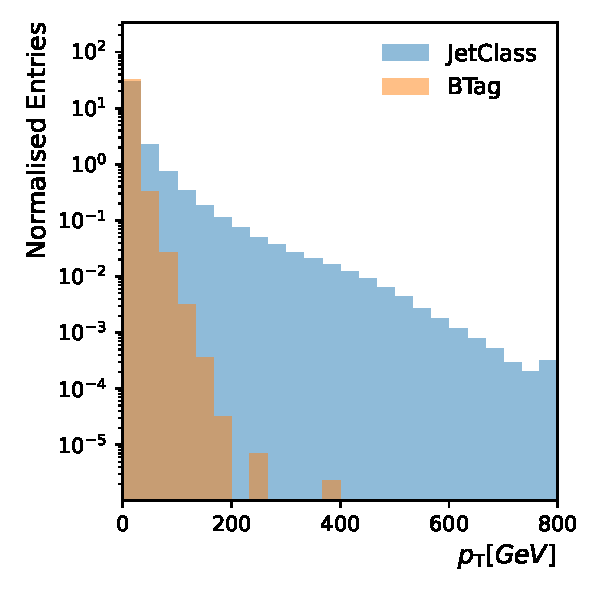
\includegraphics[width=0.32\linewidth]{Figures/foundation_models/mpm2/data/pt.pdf}
    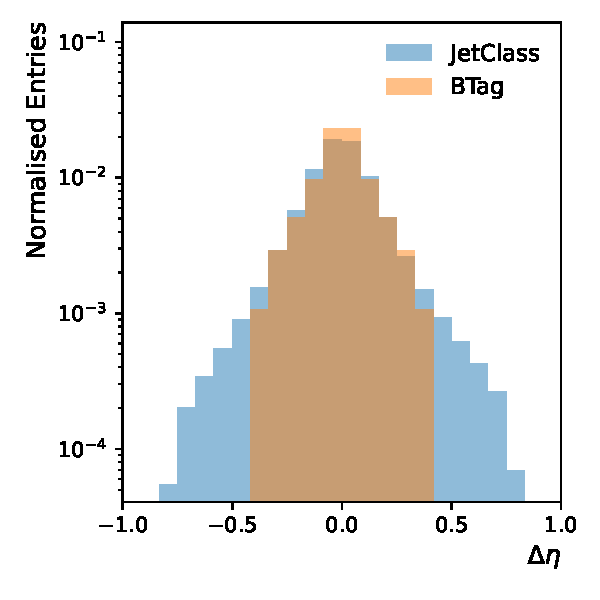
\includegraphics[width=0.32\linewidth]{Figures/foundation_models/mpm2/data/deta.pdf}
    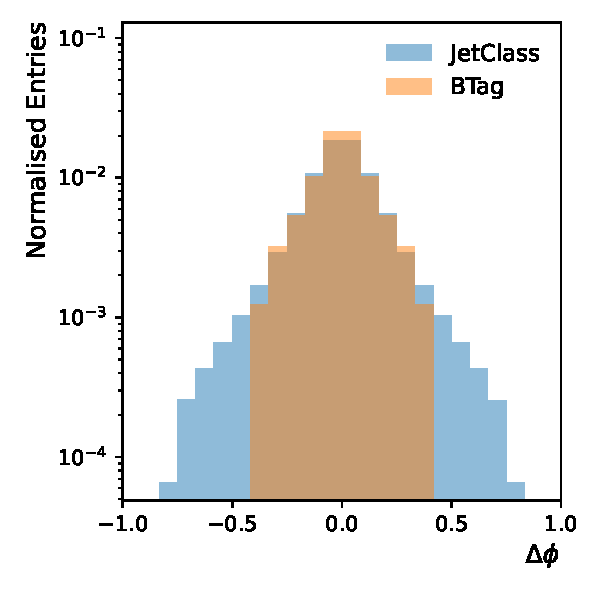
\includegraphics[width=0.32\linewidth]{Figures/foundation_models/mpm2/data/dphi.pdf}
    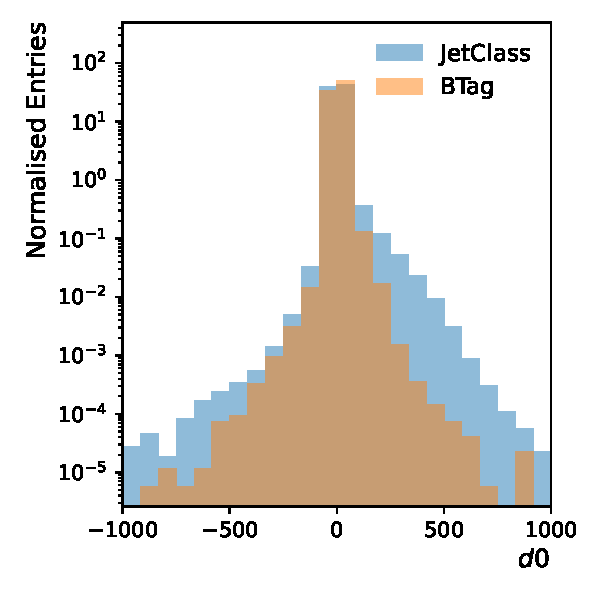
\includegraphics[width=0.32\linewidth]{Figures/foundation_models/mpm2/data/d0val.pdf}
    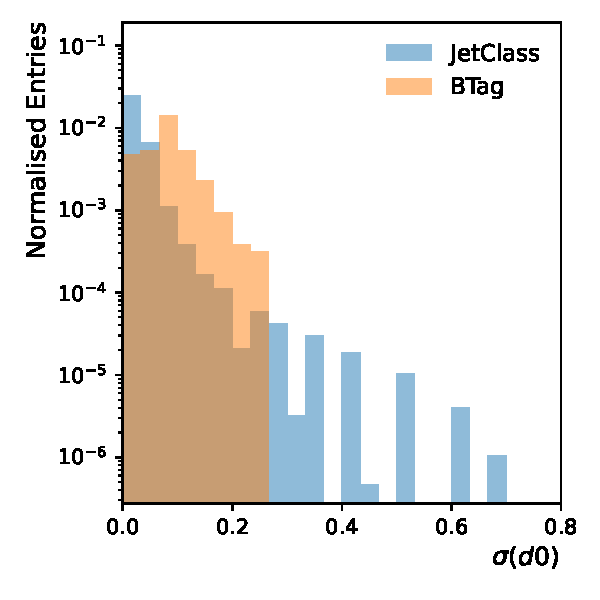
\includegraphics[width=0.32\linewidth]{Figures/foundation_models/mpm2/data/d0err.pdf}
    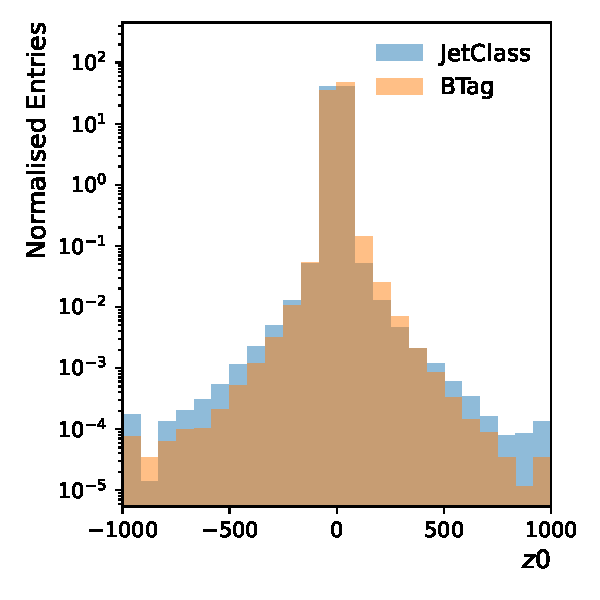
\includegraphics[width=0.32\linewidth]{Figures/foundation_models/mpm2/data/dzval.pdf}
    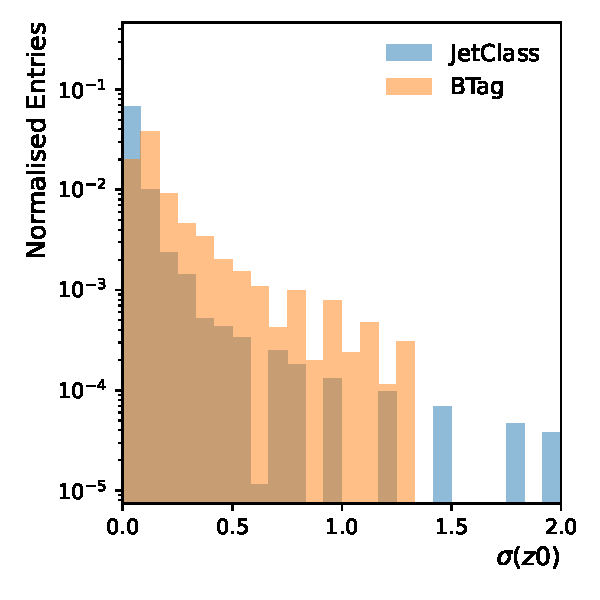
\includegraphics[width=0.32\linewidth]{Figures/foundation_models/mpm2/data/dzerr.pdf}
    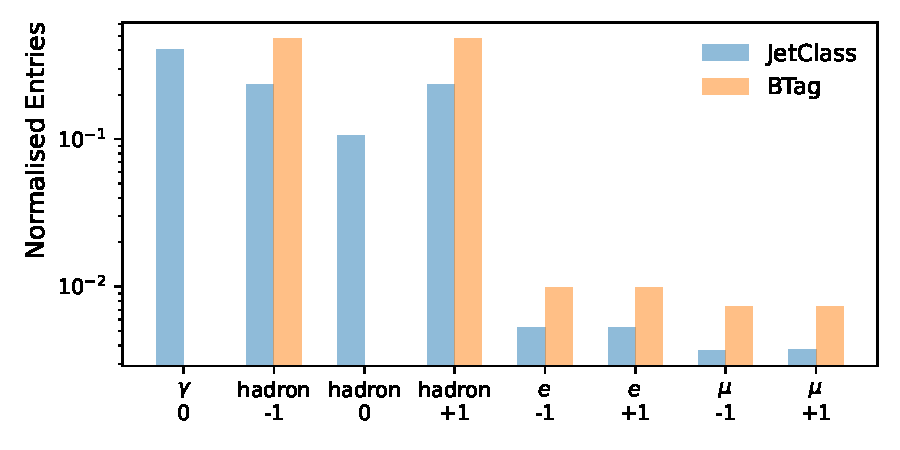
\includegraphics[width=0.64\linewidth]{Figures/foundation_models/mpm2/data/csts_id.pdf}
    \caption{The distributions of the particle features for the two datasets. The final plot shows the distributions of the particle types \xid for the two datasets.}
    \label{fig:mpm2_features}
\end{figure}

\subsection{Overview of Methods}

The various models used in this section are shown in \Cref{fig:models}.
In framing MPMv1 as a DAE, the input jet $\mathcal{X}$, its latent projection $\mathcal{Z}$, and the decoder output $\mathcal{D}$ are all sets; thus, all mappings between them must be permutation equivariant.
A transformer acts as the encoder, and a multi-layer perceptron (MLP) acts as the decoder, applied separately per set element.
APE is applied to $\mathcal{Z}$ to break the degeneracy of the masked tokens while keeping the encoder permutation equivariant.
Each element in $\mathcal{D}$ is used in a tokenized reconstruction task, where it is compared to the corresponding element of the same jet passed through the encoder of a VQVAE.

In MPMv1, the masked tokens are identical in each sublayer of the encoder, effectively adding nothing to the message-passing operations.
For MPMv2, the masked tokens are removed completely from the input set.
They are only reintroduced during decoding, resulting in $\mathcal{Z}$ having a lower cardinality than both $\mathcal{X}$ and $\mathcal{D}$.
This shifts from a model akin to BERT~\cite{BERT} to one similar to MAE~\cite{MAE}.

The decoder is also expanded to a transformer.
With a message-passing decoder, APE in the latent space provides too much information, trivializing the reconstruction task.
Therefore, APE is provided only between the masked elements, not the full jet.
This can be parameterized by a unique mask token based on the \pt~order of the dropped constituents with respect to each other only.

The loss function is derived by comparing $\mathcal{X}$ and $\mathcal{D}$ across various \textit{reconstruction tasks}.
The key differences between MPMv2 and a direct MAE re-implementation include using multiple reconstruction tasks for different feature groups and positional encoding only for the dropped set.

\begin{figure}[t!]
    \centering
    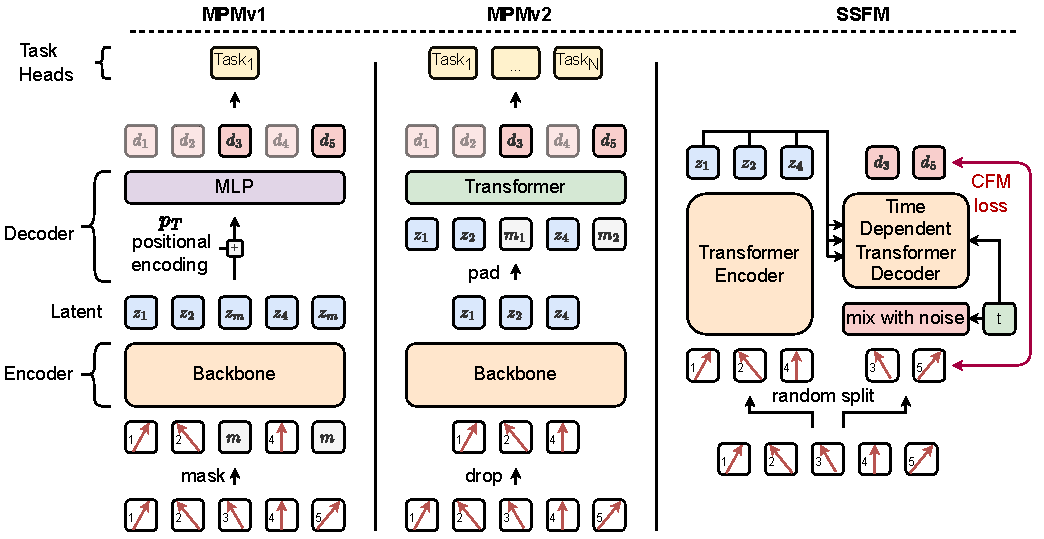
\includegraphics[width=\textwidth]{Figures/foundation_models/mpm2/FlowBert.drawio.pdf}
    \caption{(left) The original MPMv1 encoder-decoder setup compared to the new MPMv2 model (middle). The new model includes multiple reconstruction tasks, swaps the MLP decoder for a transformer, and only encodes the reduced set. (right) The Set-to-set Flow-Matching which jointly generates the dropped elements of the set using the surviving elements.
        \label{fig:models}
    }
\end{figure}

\subsection{Reconstruction Tasks}
\label{sec:recovery}

MPMv1 only uses a single VQVAE-derived reconstruction task, whereas MPMv2 combines multiple tasks to recover the continuous and categorical features separately.
Each task adds extra learnable layers (task head) and contributes to the total pre-training loss.
Each of these losses is applied per particle and only calculated for those which were masked/dropped.
One task is used specifically for the categorical feature (\xid) and five options for the continuous features (\xc) are explored.

\begin{itemize}
    \item Particle Identification: This is to recover the particle type \xid of the dropped constituent.
          It is framed as a standard classification problem, only requiring a linear layer for the task head and the cross-entropy loss function.
    \item Direct Regression: This was found insufficient for pre-training in MPMv1, but consider it worth revisiting owing to the much more powerful decoder in MPMv2.
          A linear layer is used for the task head and best results were found using the L1-loss with \xc as the target.
    \item VQVAE Tokenized Classification: This was the optimal method for MPMv1.
          A frozen VQVAE is used to construct the target indices based on \xc.
          A single linear layer is used for the task head and the cross-entropy loss function is applied.
          A new VQVAE is trained for the expanded feature list in MPMv2.
    \item K-Means Tokenized Classification: In MPMv1, similar results were observed using K-Means centroids as targets compared to VQVAE tokens.
          This is further optimized in MPMv2 by increasing the number of centroids fit on \xc to 16384.
          Like the other tasks, a single linear layer to map to this space and cross-entropy loss function are utilized.
    \item Conditional Normalizing Flow (CNF): If the strength of the tokenized form of reconstruction over regression is in learning the full posterior distribution $p(\xc_i|d_i)$ as opposed to a point estimate, then this can be achieved without the need to reframe the task as classification.
          The head is constructed using a 7-dimensional conditional normalizing flow trained on the negative log-likelihood of the continuous features given the decoder output.
    \item Conditional Flow Matching (CFM): Continuing with the idea of using generative model to conditionally generate the dropped continuous features given the surviving ones, a diffusion model is used instead of the normalizing flow.
          The head consists of an MLP conditioned on the decoder output, and trained to denoise a corrupted version of \xc via the CFM framework described in \Cref{sec:cfm}.
          The loss used is given by \Cref{eq:linear_cfm_loss}.
\end{itemize}

\subsection{Set-to-Set Flow Matching}

In addition to MPMv2, another new model is introduced which is labelled as Set-to-Set Flow-Matching (SSFM) is shown in \Cref{fig:models}
This uses a time-dependent transformer decoder to generate constituents from latent nodes.
The approach is similar to the diffusion-masked autoencoder from CV~\cite{diffmae}.
During the masking the input set $\mathcal{X}$ is split into a reduced set $\mathcal{S}$ of size $M$ and its complement $\mathcal{T}$.
The reduced set passes through the encoder to obtain the latent set $\mathcal{Z}$, which is then used in the decoder's cross-attention layers.
The decoder is trained as a set-CFM model to generate $\mathcal{T}$.

The training task of denoising prevents any degeneracy, eliminating the need for APE or mask tokens.
Furthermore, adjusting the masking rate $D_f$ controls fraction of the jet which is sent to the encoder, and which is sent to the decoder.
When $D_f=1.0$, the decoder functions as a full generative model.
Thus, this pre-training setup facilitates the creation of a backbone for conventional downstream tasks, as well as a decoder which could be used as a generative model, similar to those described in \Cref{ch:jet_generation}.
During training, sampling $D_f \sim \mathcal{U}(0.2, 1.0)$ balances these objectives.

\subsection{Model Architecture}

Several changes to the original MPMv1 model are made.
The Normformer architecture is replaced with a more standard pre-norm encoder with 8 layers, each with a 512-embedding dimension.
Eight heads are used for the self-attention layers.
Inside the transformer the MLPs have a hidden dimension of 1024 and used the SwiGLU activation function~\cite{SwiGLU}.
LayerScale~\cite{GoingDeeper} is used for all residual updates.
The decoder used in the MPMv2 models uses the same layer types as the backbone, but is considerably smaller, with only four layers and a model dimension of 256.
Some of the experiments include eight register tokens~\cite{VisionTransformersNeed} to store global information in the encoder.

Models are trained with the AdamW optimizer with a weight decay of $1 \times 10^{-5}$.
The learning rate increases linearly for the first 50k steps up to $1 \times 10^{-3}$ and then decays exponentially with a 100k half-life.
Pre-training is conducted on the full JetClass training set with a batch size of 1000.

Each task head introduces new layers.
Most of these are simple affine layers to map the latent space to the target space.
The exceptions to this are the CNF and CFM tasks.
For the flow, six coupling layers with rational quadratic spline transformations are used.
Each coupling layer contains a two-layer MLP with 128 hidden units as the conditioner.
The transformation is conditioned on the decoder outputs by concatenating them to the input of each MLP.
The CFM head uses a three-layer MLP with a hidden dimension of 256.
The inputs to this model are the partially noised targets ${\xc_i}(1 - t) + \z t$, the decoder outputs for the particle $d_i$, and the diffusion time $t$.

For the SSFM model, a transformer decoder is used with four layers, eight heads, and a model dimension of 256.
The SSFM decoder has more parameters than the MPMv2 decoder due to the additional cross-attention layers.
A linear layer maps the latent space to the 256 for these cross-attention operations.
The method described in \textcite{DIT} is used for time injection.

\subsection{Experiments}
\label{sec:mpm2_experiments}

The initial experiments in this section investigate the impact of the new model design compared to the original MPMv1.
This is followed by a full comparison of reconstruction strategies using the performance of the backbone on the new downstream task test bed.

Several MPMv2 backbones are pre-trained using the using one of the \xc reconstruction tasks (which it is labelled by) and the classification task for \xid.
A SSFM model is also trained.
Pre-training is run for 1M steps, after which specific downstream task layers are appended to the backbone, and the model is fine-tuned.
All fine-tuning is run for 200k steps with a batch size of 500, allowing for early-stopping using a validation set.
A randomly initialized network, trained ``From Scratch'' is used as a baseline to highlight the performance provided by pre-training.
Each experiment is repeated 5 times to estimate the run-to-run variance.

Fine-tuning performance is greatly enhanced over MPMv1 using a specific scheduler for the backbone learning rate.
This scheduler is defined by two parameters: the number of frozen-steps and the number of warmup-steps.
At the start of training, the backbone is frozen, which allows the new head to adapt.
Then, the backbone learning rate catches up to the head learning rate linearly over the warmup-steps.
After this the backbone and head learn together.

\subsubsection{Ablation Studies}

To evaluate the proposed changes to the model, a simple metric is required.
This is chosen to be the accuracy of an in-distribution classifier on the test on the JetClass dataset.
For these studies only, pre-training is limited to 200k steps.
Pre-training is performed using the regression or K-Means tasks for \xc.
After this, the backbone is frozen and a classifier-head made from two class-attention layers~\cite{GoingDeeper}, is appended.
These new layers are trained for 200k steps using cross-entropy loss.
The results of this ablation study are shown in \Cref{tab:construction}.

Initially, the original training setup of MPMv1, which used a masking rate of $D_f=0.3$, is replicated.
The first modification is the updated transformer layers.
This is followed by the addition of the impact features to the particle attributes.
Next the particle ID feature is added, and the ID reconstruction task is combined with the continuous tasks.
All of these changes improves the accuracy of the backbone, from $56.2\%$ to $74.0\%$ when using K-Means for the reconstruction task.

The subsequent change is the replacement of the MLP decoder with a transformer.
This change significantly improves the performance of the backbone, narrowing the gap between the K-Means and regression pre-training methods.
To verify the impact of the decoder change, the experiment is rerun using the regression and the new transformer layers, but without the impact parameters, particle ID inputs, or particle ID task.
This model achieves an accuracy of 65.0\%, an increase of 9.5\%.
An additional advantage of adopting the MAE setup is achieving a 40\% reduction in GPU memory usage due to the reduced point cloud size passed to the encoder and the use of non-padded representations of the batch~\cite{FlashAttentionFastMemoryEfficient}.
The total inference time also improves by approximately 15\%.

The following change is the addition of registers to the encoder~\cite{VisionTransformersNeed}.
Registers prevent the transformer from overwriting nodes with global information, increasing performance with minimal computational cost.
This improves the accuracy of the backbone marginally.

At this stage, the mask rate $D_f$ and decoder depth is optimized, and the results are shown in \Cref{fig:sweep}.
They both use the K-Means + ID setup.
They are optimized separately, with the decoder depth sweep using $D_f=30\%$ and the $D_F$ sweep using a depth of 2.
The model is observed to be relatively robust to the mask rate, with values as high as $D_f=90\%$ still resulting in a classification accuracy of over 80\%.
The optimal mask rate is determined to be $D_f=40\%$.
Increasing the decoder depth improves performance, but only four layers are tested due to computational constraints.
It is expected that further improvements could be made with a deeper decoder.
These optimal values are used for the final model, which is trained for 1M steps.

\begin{table}[t]
    \centering
    \caption{The effects of the model redesign on the accuracy of a classifier head trained using the encoder outputs. All models except the final iteration are pre-trained using 200k steps, a 2-layer decoder, and $D_f=30\%$.
    }
    \label{tab:construction}
    \begin{tabular}[t]{lrlrl}
        \toprule
                                                                & \multicolumn{2}{l}{Regression} & \multicolumn{2}{l}{K-Means}                   \\
        \midrule
        MPMv1 using $(\pt, \eta, \phi)$                         & 48.9                           &                             & 56.2 &          \\
        + updated transformer layers                            & 55.5                           & \im{6.6}                    & 62.2 & \im{6.0} \\
        + impact parameter features                             & 62.2                           & \im{6.7}                    & 70.2 & \im{8.0} \\
        + constituent ID feature and ID reconstruction task     & 63.5                           & \im{1.3}                    & 74.0 & \im{3.8} \\
        + transformer as decoder (MAE)                          & 79.2                           & \im{15.7}                   & 81.4 & \im{7.4} \\
        + registers                                             & 80.4                           & \im{1.2}                    & 83.0 & \im{1.6} \\
        + longer train (1M steps) + deeper decoder + $D_f=40\%$ & 83.3                           & \im{2.0}                    & 84.0 & \im{1.0} \\
        \bottomrule
    \end{tabular}
\end{table}

\begin{figure}[htp!]
    \centering
    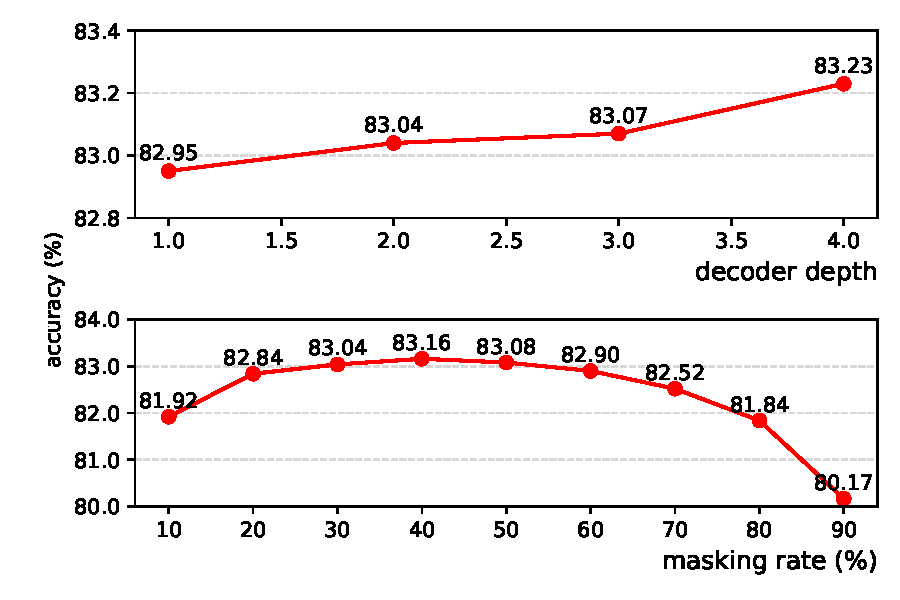
\includegraphics[width=0.7\linewidth]{Figures/foundation_models/mpm2/sweep.pdf}
    \caption{The effect of the decoder depth (top) and the mask rate (bottom) on the classification accuracy using the outputs produced by an MPMv2 backbone trained with the K-Means and ID tasks.}
    \label{fig:sweep}
\end{figure}

\subsubsection{In-Distribution Classification}

Classification is performed on the JetClass dataset using the same classifier head as described in the above ablation studies.
Data efficiency of the backbone is assessed by varying the number of jets used for supervised training from 1k to 100M, as shown in \Cref{fig:jetclass}.
For the 100M sample, all jets in the JetClass training set are used, but 200k steps limits the training to one epoch.
At each training set size, pre-trained backbones outperform the randomly initialized network, although the performance boost decreases with the number of jets.
At 100M jets, accuracy ranges between $85.0\%$ (regression) and $85.3\%$ (K-Means), compared to $84.3\%$ for random initialization.
The K-Means backbone excels with more data, while CNF and Regression backbones are more data-efficient.
The CNF backbone fine-tuned on 10k jets matches the performance of a network trained from scratch with 1M jets.

For this task on the JetClass dataset, the state-of-the-art model is ParT~\cite{ParticleTransformerJet}.
It employs a similar transformer-based architecture, but also utilizes additional edge features.
Training also proceeds for 1M batches, which is over 470 times longer than the combined pre-training and fine-tuning of the MPMv2 models.
The final accuracy is $86.1\%$, which is only slightly higher than the best MPMv2 backbone.

\subsubsection{Weakly Supervised Classification}

The CWoLa setting is emulated using the same methodology as in MPMv1 and use the same classifier head as the previous experiments.
In \Cref{fig:cwola}, the SIC is shown at a background rejection rate of $r_b=99\%$ for classifiers on a test set containing pure samples of QCD background and top signal.
The pre-trained backbones considerably outperform the benchmark.
The Regression backbone requires only 500 top jets present in the training set to achieve an SIC of 8.18.

\begin{figure}[h!]
    \centering
    \begin{subfigure}{0.4\linewidth}
        \centering
        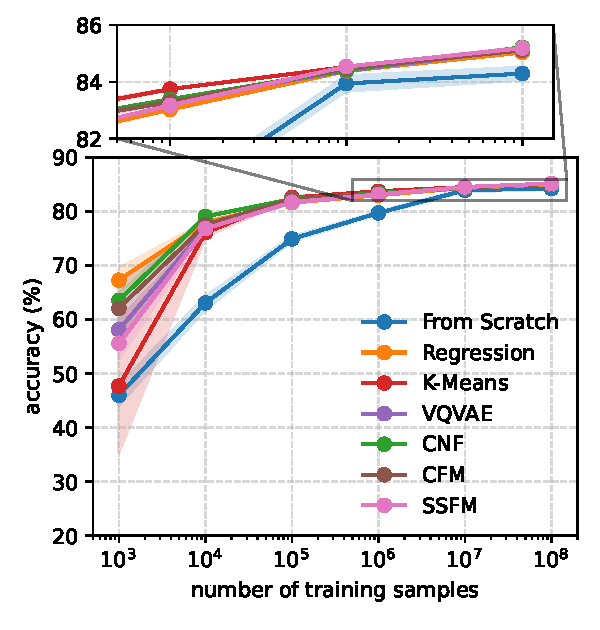
\includegraphics[width=\linewidth]{Figures/foundation_models/mpm2/final/jetclass_finetune.pdf}
        \caption{}
        \label{fig:jetclass}
    \end{subfigure}
    \begin{subfigure}[b]{0.4\textwidth}
        \centering
        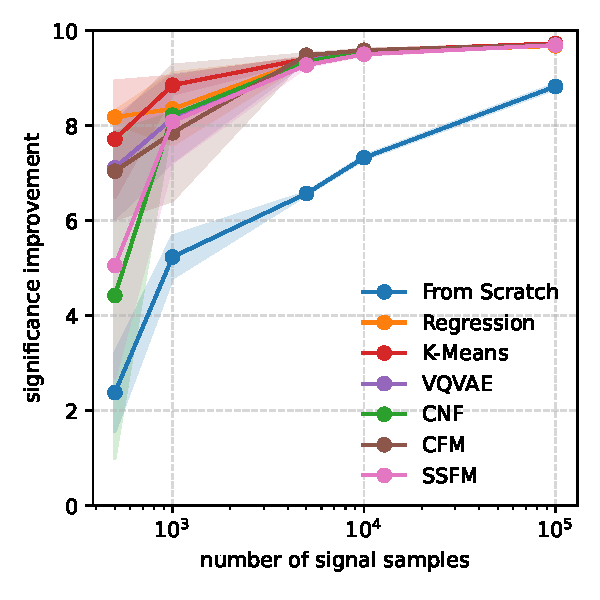
\includegraphics[width=\linewidth]{Figures/foundation_models/mpm2/final/cwola_finetune.pdf}
        \caption{}
        \label{fig:cwola}
    \end{subfigure}
    \caption{The in-distribution performance of the fine-tuned models on the JetClass dataset. \subref{fig:jetclass} shows the accuracy using standard supervised classification as a function of the dataset size. \subref{fig:cwola} shows the significance-improvement of the models trained in a CWoLa setting as a function of the number of signal samples in the dataset.}
    \label{fig:plot_A}
\end{figure}

\subsubsection{Out-of-Distribution Classification}

The performance of backbones in classifying the BTag dataset, which comprises lower-energy, narrower jets with a few charged particles, is tested.
As shown in \Cref{fig:btag}, the accuracy of the three-class classifier is presented as a function of the number of jets used for training.
All pre-trained backbones surpass the benchmark initialization, demonstrating the generalizability of the learned mappings beyond JetClass or fat jets.
The CNF backbone achieves the highest performance in this task, but all pre-trained backbones converge at approximately 70\% accuracy with the maximum number of jets.

\subsubsection{Secondary Vertex Finding}

A track vertex denotes a common point from which reconstructed particle tracks originate, indicating the location of an interaction or decay.
Bottom and charm hadrons produced in the collision travel several millimetres beyond the interaction point before decaying, resulting in multiple vertices within the same jet.
These vertices are crucial for identifying heavy-flavour jets, as discussed in \Cref{ch:spice}.
Kaon decays also contribute additional vertices.
This task is recast as an edge classification problem, where pairs of tracks are classified as positive or negative.
This task is similar to instance segmentation in CV, where the goal is to segment the image into unique instances of different objects.
There are $N(N-1)/2$ unique pairs to evaluate for a jet with N tracks.

The additional layers for this task follow a twin-network approach~\cite{siamese}, where the probability that two tracks $x_i$ and $x_j$ originate from the same vertex is defined by $\sigma\left(G\left[|F\left(z_i\right)-F\left(z_j\right)|\right]\right)$, with $G$ and $F$ being MLPs, $z_i$ and $z_j$ as backbone outputs, and $\sigma$ as the sigmoid function.
The adjusted Rand index (ARI)~\cite{ari}, as used by \textcite{SecondaryVertexFinding}, is the designated performance metric.
The ARI is plotted against the number of secondary vertices in \Cref{fig:vtx}.
The backbone trained with the CNF task performs best, although all backbones surpass the benchmark.

\subsubsection{Heavy Track Identification}

The final task involves identifying the vertex type associated with each track.
It resembles the track origin auxiliary task in \Cref{ch:spice} and also draws parallels with the semantic segmentation task in CV.
Tracks in the BTag dataset can be linked to a displaced $b$-quark decay, $c$-quark decay, the primary vertex, or some other source (kaon decay, etc.).
The task head is a straightforward three-layer MLP appended to the backbone, acting on each constituent independently.
Due to the heavily imbalanced class distributions, balanced accuracy is the preferred metric for distinguishing between pre-training methods.
As shown in \Cref{fig:trk}, balanced accuracy is plotted as a function of the number of tracks in each jet, with pre-trained backbones consistently outperforming the baselines.

\begin{figure}[h!]
    \centering
    \begin{subfigure}{0.32\linewidth}
        \centering
        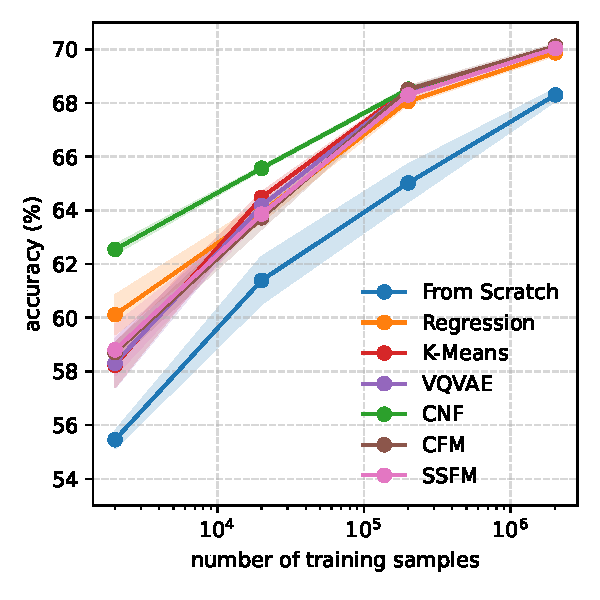
\includegraphics[width=\linewidth]{Figures/foundation_models/mpm2/final/btag_finetune.pdf}
        \caption{}
        \label{fig:btag}
    \end{subfigure}
    \begin{subfigure}[b]{0.32\textwidth}
        \centering
        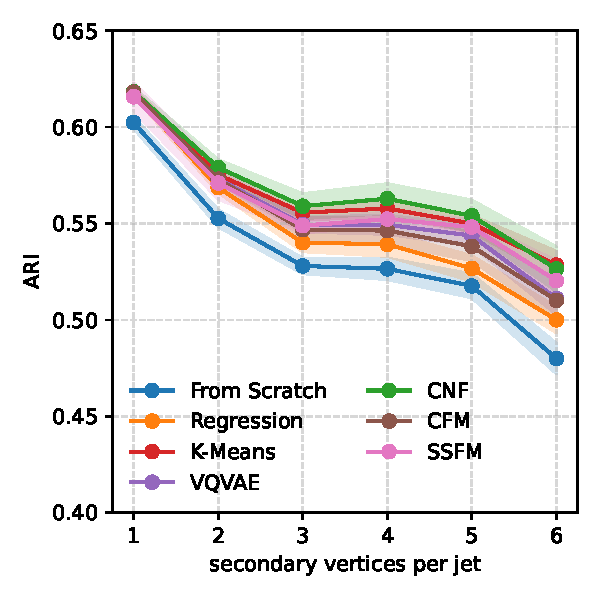
\includegraphics[width=\linewidth]{Figures/foundation_models/mpm2/final/vtx_finetune_ari.pdf}
        \caption{}
        \label{fig:vtx}
    \end{subfigure}
    \begin{subfigure}[b]{0.32\textwidth}
        \centering
        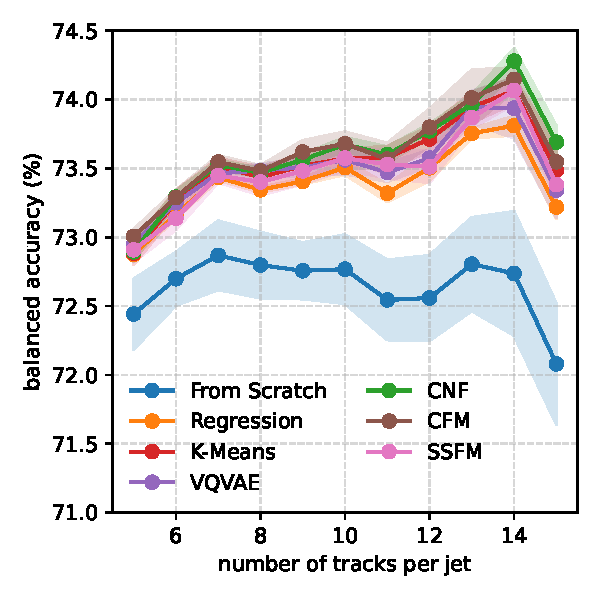
\includegraphics[width=\linewidth]{Figures/foundation_models/mpm2/final/trk_finetune.pdf}
        \caption{}
        \label{fig:trk}
    \end{subfigure}
    \caption{The performance of the fine-tuned models on the BTag dataset. \subref{fig:btag} shows the supervised jet classifier accuracy versus the number of samples used in fine-tuning.
        \subref{fig:vtx} shows the ARI score for the segmentation task versus the number of secondary vertices within each jet. \subref{fig:trk} shows the balanced accuracy for the track identification task as a function of the number of tracks in each jet.}
    \label{fig:plot_B}
\end{figure}

\section{Conclusion}
\label{sec:conclusion}

This study aims to build upon MPMv1's findings, in part by assessing the necessity of the costly tokenization step in pre-training.
Alternative reconstruction methods are explored, such as simpler tokenization through the K-Means algorithm and conditional generative models.
Additionally, a novel pre-training method using set-to-set generation is introduced, proving to be competitive with MPMv2.
The new models significantly outperform an untrained backbone and the original MPMv1 in various tasks, including those involving out-of-distribution data.
However, the differences between these pre-training strategies were minimal.
A key improvement is the implementation of a more powerful decoder.
These findings suggest tokenization is not essential, which may have implications for other SSL models using VQVAE, such as \textcite{Omnijet}.

Despite the promising results, the self-supervised training strategies for particle physics jets face several limitations.
All experiments are conducted using the parametric \delphes fast simulation package, which does not fully replicate the complexity of real-world data.
The next significant step would be transitioning to real data and full simulations.
The approach is confined to jets and a few relevant downstream tasks, but another extension would be to move to full event-level data.
This would increase the expected set size from $O(100)$ to $O(1000)$, necessitating substantially more computation due to the transformer architecture and addressing these challenges is a key area for future work.
